\documentclass[10pt,twocolumn,letterpaper]{article}

\usepackage{cvpr}
\usepackage{times}
\usepackage{epsfig}
\usepackage{graphicx}
\usepackage{amsmath}
\usepackage{multirow}
\usepackage{amssymb}
\usepackage{lscape}
\usepackage[table,xcdraw]{xcolor}


% Include other packages here, before hyperref.
\usepackage{float}
\usepackage{enumitem}

% If you comment hyperref and then uncomment it, you should delete
% egpaper.aux before re-running latex.  (Or just hit 'q' on the first latex
% run, let it finish, and you should be clear).
\usepackage[breaklinks=true,bookmarks=false]{hyperref}

\cvprfinalcopy % *** Uncomment this line for the final submission

\def\cvprPaperID{****} % *** Enter the CVPR Paper ID here
\def\httilde{\mbox{\tt\raisebox{-.5ex}{\symbol{126}}}}

% Pages are numbered in submission mode, and unnumbered in camera-ready
%\ifcvprfinal\pagestyle{empty}\fi
\setcounter{page}{1}
\begin{document}

%%%%%%%%% TITLE
\title{Using respiratory sounds to detect presence of Chronic Obstructive Pulmonary Diseases with Machine Learning}

\author{\textbf{Aryaman Trivedi, Divyajeet Singh, Ieshaan Awasthy, Palaash Goel}\\
\textit{Dept. of Computer Science and Engineering}\\
Indraprastha Institute of Information Technology Delhi, India\\
{\tt\small \{aryaman21022, divyajeet21529, ieshaan21054, palaash21547\}@iiitd.ac.in}
}


\graphicspath{{Assets/}}

\maketitle


\begin{abstract}
    Chronic Obstructive Pulmonary Diseases (COPDs) are a group of diseases that cause breathing-related problems
    and affect millions of people worldwide. COPDs are
    usually diagnosed by auscultation - the process of listening to organ sounds for diagnosis. However, this requires extensive
    experience and is prone to human error. In this paper, we propose a machine learning-based solution to detect
    COPDs using respiratory sounds. Our machine-learning model detects COPDs as accurately as the most experienced medical professionals. \\
    We use a dataset of 920 annotated audio samples collected from 126 subjects. This paper presents an analysis of models we tried to solve this problem. We achieved an accuracy score of $\textbf{0.8967}+$ using our top-performing model, exceeding the accuracy of most medical professionals.
\end{abstract}

%-------------------------------------------------------------------------
\section{Motivation}

Motivated to solve a real-world problem, the authors focused on the medical domain due to its profound
health implications. Minor mistakes by medical professionals may manifest as life-lasting health effects.
Exploring areas where such issues can be mitigated led us to the problem of detecting COPDs.

Detecting COPDs is a crucial task requiring extensive experience in auscultation - listening to the sounds of
organs such as the heart and lungs to help find a medical diagnosis. However, Kim \etal \cite{kim} found a
significant lack of accuracy in detecting COPDs among professionals. Most medical professionals, including resident doctors, detect COPDs with an
average accuracy of only 61\%, except fellows who exhibit an accuracy of 84\%. This misdiagnosis of COPDs can lead to
a significant increase in medical emergencies and a higher risk of mortality, as the patients' actual
conditions remain untreated, as noted by Diab \etal \cite{diab}.

To address this problem, we have provided an ML-based solution that can accurately detect COPDs using respiratory sounds. By doing so, we aim to improve the quality of care for patients with respiratory
diseases and reduce the risk of misdiagnosis while reducing the stress on healthcare systems.

%-------------------------------------------------------------------------
\section{Introduction: Problem Statement}
As mentioned previously, medical practitioners severely lack the ability to accurately diagnose chronic obstructive
pulmonary diseases due to the skill and difficulty associated with auscultation. This challenge can be tackled
with a machine learning-based solution that can reliably detect COPDs accurately using respiratory sounds.
Medical professionals can use the solution to aid their diagnosis.

%-------------------------------------------------------------------------
\section{Literature Review}

\begin{enumerate}
    \item
    \href{https://www.nature.com/articles/s41598-021-96724-7}{Respiratory sound classification for crackles,
    wheezes, and rhonchi in the clinical field using deep learning by Kim \etal}

    Studies the performance of medical professionals and CNNs in detecting COPDs from 1918 auscultation sounds
    collected from 831 patients. The authors split the audio into 6-second clips with 50\% overlap and generated
    variations of Mel-Spectrograms as inputs for the CNN. They found that a frozen VGG16 trained on the ImageNet
    dataset (frozen transfer learning) for feature extraction, followed by a single convolution layer for
    classification, performed with an accuracy of 86.5\%. They also found that medical students, interns, and
    residents struggle to identify COPDs, and only fellows could accurately detect COPDs from audio.

    \item
    \href{https://www.ncbi.nlm.nih.gov/pmc/articles/PMC7959628/}{Deep learning based respiratory sound analysis for
    detection of chronic obstructive pulmonary disease by Srivastava \etal}

    Uses CNNs and DL methods with 10-fold cross-validation to provide a rigorous analysis of 920 annotated audio
    samples collected from 126 subjects for COPD detection. The authors compared various features generated
    from the samples using the Librosa python library, including Mel-Spectrograms and Chromagrams. Their system
    also attempts to interpret the severity of the disease identified, such as mild, moderate, or acute, with an
    ICBHI score of 93\%. The authors find that Mel-Frequency Cepstral Coefficients (MFCCs) provided better accuracy
    in detecting COPD than other features.

    % \item
    % \href{https://www.researchgate.net/publication/354521576_MosAIc_A_Classical_Machine_Learning_Multi-Classifier_Based_Approach_against_Deep_Learning_Classifiers_for_Embedded_Sound_Classification}
    % {MosAIc: A Classical ML Multi-Classifier Based Approach against Deep Learning Classifiers for
    % Embedded Sound Classification by Lhoest et al}

    % Outlines various ML techniques useful for audio classification and performs a comparative survey between them by performing a
    % classification task on various environmental sound recognition datasets. These techniques can be used as a baseline
    % for our project while also giving us the flexibility to explore different methodologies of achieving a well-performing model.
\end{enumerate}

This study sheds light on some potential paths for us to take for our machine-learning models and feature
extraction. Further, they provide domain knowledge of other authors and help us understand the data better.

%-------------------------------------------------------------------------
\section{Dataset}
The \href{https://ai4eu.dei.uc.pt/respiratory-sounds-dataset/}{Respiratory Sound Database} provided by \cite{rocha}
is a collection of annotated audio samples collected independently over several years by two research teams from the
the University of Coimbra \& the University de Aveiro, Portugal, and the Aristotle University of Thessaloniki, Greece.

The dataset contains 920 samples annotated by respiratory experts recorded from 126 subjects spanning all age
groups using heterogeneous recording devices. There are a total of 5.5 hours of clean and noisy recordings
containing 6898 respiratory cycles - 1864 contain crackles, 886 contain wheezes, and 506 contain both.

\subsection*{Data Compilation}
Despite its diversity, the size of the dataset is very limited, mainly when limited to numerical values from the 126 patients. Demographic data for these patients was extracted from a plain text file from the dataset.

\subsubsection*{Numerical Data}
The 920 recordings have been taken from multiple microphones in different locations for varying durations. Most patients don't have recordings in every configuration, while others have recordings with duplicate configurations. The configurations for each recording were encoded within the filename. For example, \texttt{101\_1b1\_Al\_sc\_Meditron.wav} corresponds to patient number \texttt{101}, recording index \texttt{1b1}, taken in the Left Anterior (\texttt{Al}) location, in single channel mode (\texttt{sc}), using the Meditro Stethoscope. The annotations for each respiratory cycle (cycle\_beginning\_time, cycle\_ending\_time, crackles\_present, wheezes\_present) were contained in the same folder with the same name as the recording in plain text format, as shown below:
\vspace*{0pt} \\
\hspace*{75pt} \texttt{0.036    0.579	0	0} \\
\hspace*{75pt} \texttt{0.579	2.450	0	0} \\
\hspace*{75pt} \texttt{2.450	3.893	0	0}

We attempted to create a single numerical dataset by compiling each patient's data into a percentage value for each chest location. Models trained on this dataset are treated as baselines for our future models.
% We compiled the data for each patient into percentage values corresponding to each chest location. Thus, we generated the 12 columns of the form \texttt{[percent\_\{whseeze/crackle\}\_\{location\}]}.

% Finally, audio visualisations were generated using the Librosa library. Data was loaded for the entire clip and for the first cycle corresponding to the required parameters (no crackles/wheezing, crackles but no wheezing, wheezing but no crackles, or both), sourced from the text files. Mel Frequency Spectrograms and Mel-Frequency Cepstral Coefficients (MFCCs) were generated for each of these clips since we expect these to be relevant to our future models based on our literature survey.

A disadvantage to this approach was temporal invariance - by compressing all the breathing cycles into a singular number (representing the proportion of cycles where crackling or wheezing was detected, averaged across multiple recordings), we lost potentially relevant data about ordering these cycles. We also lost the single/multi-channel data in the process, although the loss should not affect our numerical predictions.

\subsubsection*{Audio Data}
To address the disadvantages, we utilize four techniques. A set of features from audio files was generated using Mel Frequency Spectrograms and MFCCs, which capture the power distribution of frequencies in the signal for each phenome of a sound. Being scaled on the mel frequency scale allows them to accurately mimic human perceptions of sound. Mel Spectrograms carry many of the same advantages as MFCCs, but provide a detailed representation of the frequency content of an audio signal and provide sharper resolution. \\
More feature maps were generated, specifically using Chromagrams, representing energy distribution across the twelve pitch classes in Western music, and Chroma-Energy Normalized Statistics (CENS), which smooth out local deviations in audio features such as pitch and articulation. \\
This way, we end up with four different feature maps to train models on. These techniques of audio-feature extraction have been studied extensively in \cite{srivastava}.

\begin{figure}[htbp]
    \centerline{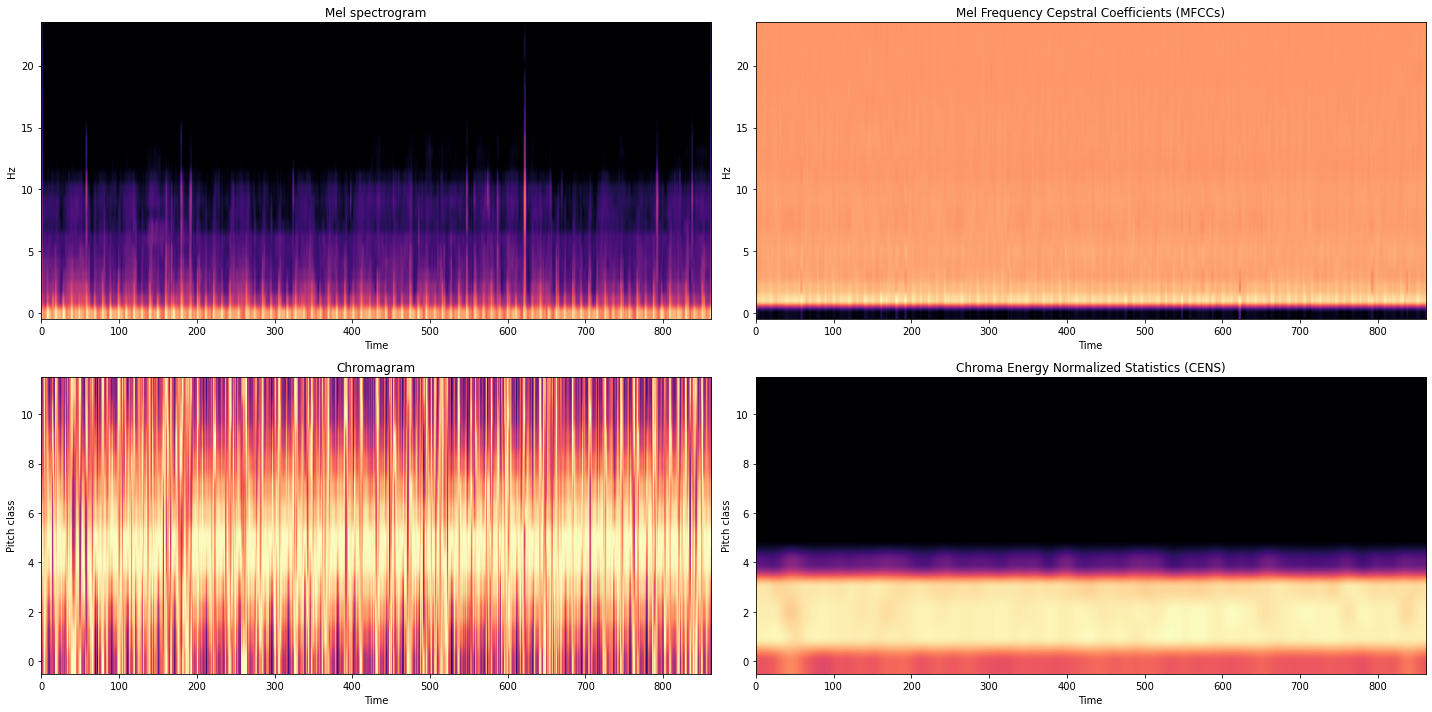
\includegraphics[width=0.45\textwidth]{compiled_original.png}}
    \caption{Discriminatory Features Extracted from Audio Files}
    \label{fig:aud_feet}
\end{figure}

\subsubsection*{Preprocessing}
Audios were clipped or padded to 20 seconds each. We perform augmentation on the dataset to increase the robustness of the trained model, deal with the problem of our limited dataset, and artificially generate more (and varied) training samples. The techniques of time shifting, pitch shifting, time stretching, and adding random noise were used for augmentation. The preprocessing introduces some degree of invariances with respect to time and pitch in the extracted features.

\subsection*{Data Analysis and Visualization}
An exploratory data analysis determined features relevant to training an optimal model. Firstly, the distribution of the demographics revealed that most data points in the dataset corresponded to adults, most of whom were unhealthy. Hence, it became apparent that to scale up the project, separate models may be needed to predict the presence of COPDs in children and adults.
\begin{figure}[htbp]
    \centerline{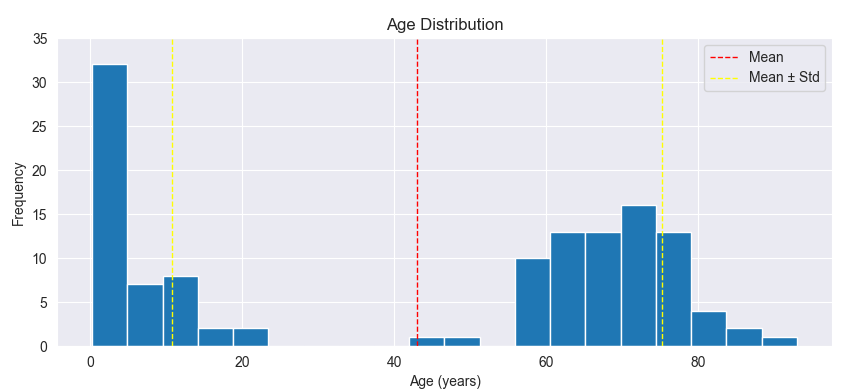
\includegraphics[width=0.45\textwidth]{age_hist.png}}
    \caption{Distribution of Age}
    \label{fig:age_hist}
\end{figure}

In fact, BMI is not defined for children, and the heights and weights of children were given in the dataset.
% These features were strongly correlated, as shown in Figure \ref{fig:weight_height}.
% \begin{figure}[htbp]
%     \centerline{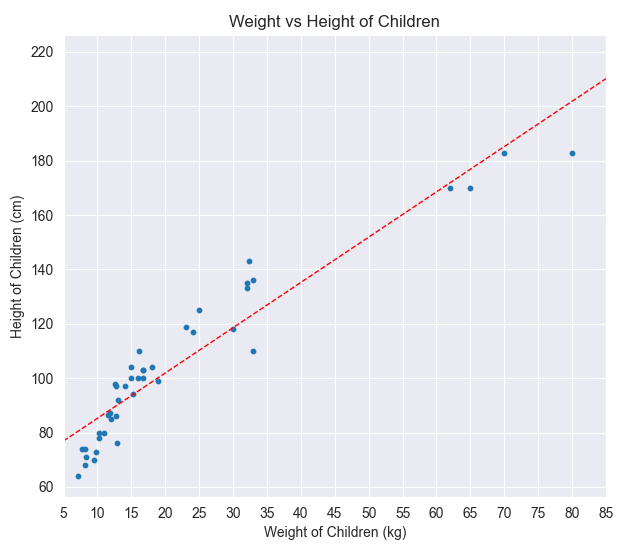
\includegraphics[width=0.4\textwidth]{weight_height.png}}
%     \caption{Distribution of Weight vs height (Children)}
%     \label{fig:weight_height}
% \end{figure}

% Figure \ref{fig:corr} shows the correlation of different features of the numerical data. It is clear that some features like \texttt{percent\_wheeze\_Ar} show little to no correlation with others, some show a slight positive correlation, and others like \texttt{age} show some negative correlation.
% \begin{figure}[htbp]
%     \centerline{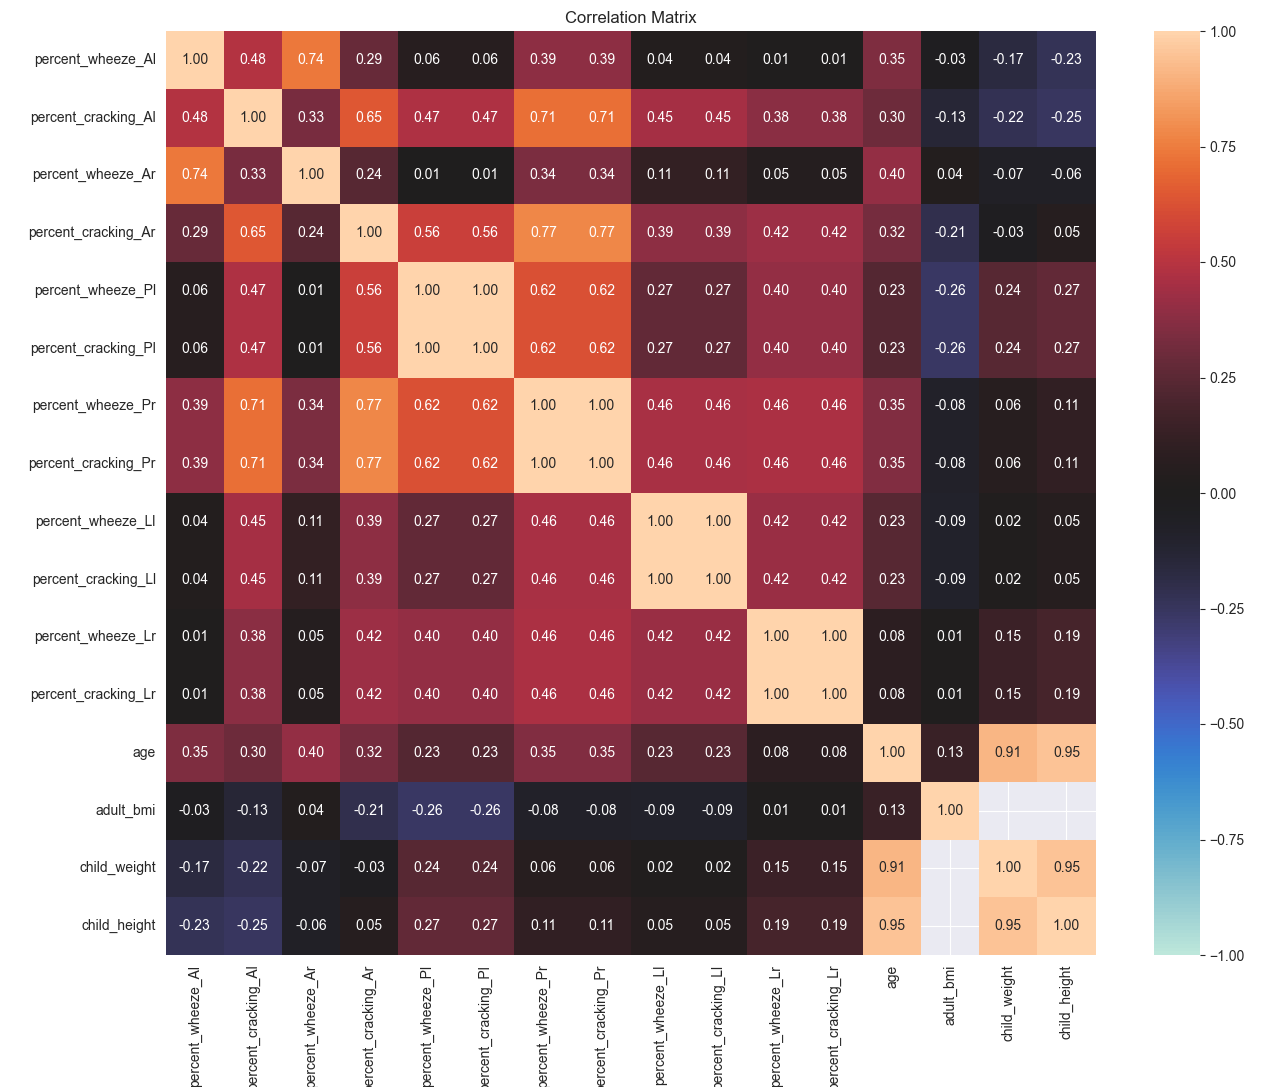
\includegraphics[width=0.5\textwidth]{corr.png}}
%     \caption{Correlation Matrix}
%     \label{fig:corr}
% \end{figure}

The distribution of the diseases present in the database strongly suggests that the database is imbalanced. Most adults were found to be unhealthy -
most of them had general COPD, while the distribution was roughly equal for children.
\begin{figure}[htbp]
    \centerline{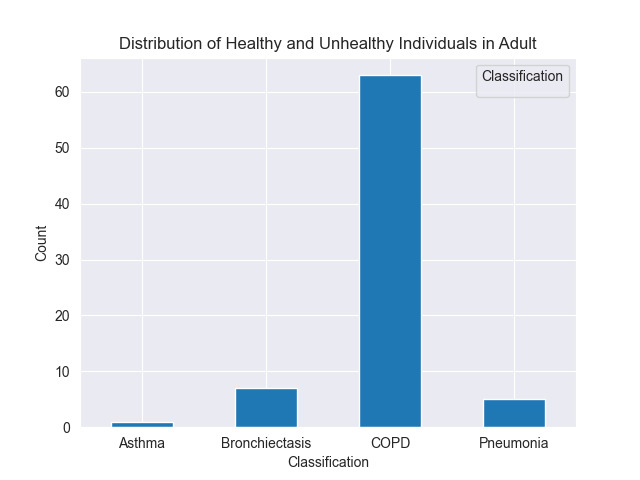
\includegraphics[width=0.35\textwidth]{adult_unhealthy.jpg}}
    \caption{Distribution of specific COPDs in Adults}
    \label{fig:adult_unhealhty}
\end{figure}

Finally, a distribution of the percentage of cracking and wheezing in respiration was drawn, classifying the patients as healthy and unhealthy. As expected, the highest mean of both was displayed by unhealthy adults. This clearly indicates that these sounds are good discriminating features, at least to classify whether a person is healthy.
\begin{figure}[htbp]
    \centerline{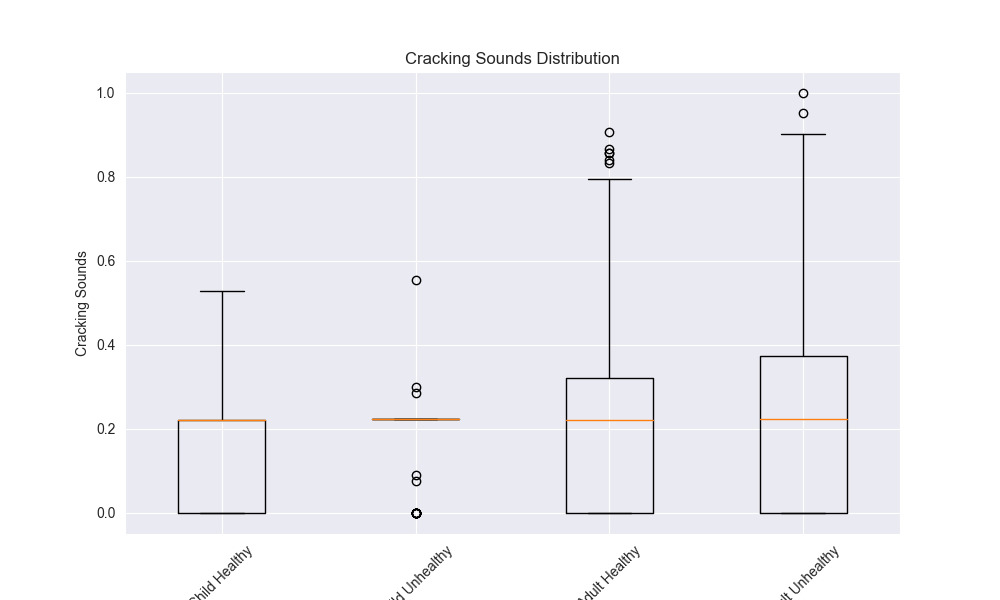
\includegraphics[width=0.35\textwidth]{cracking.jpg}}
    \centerline{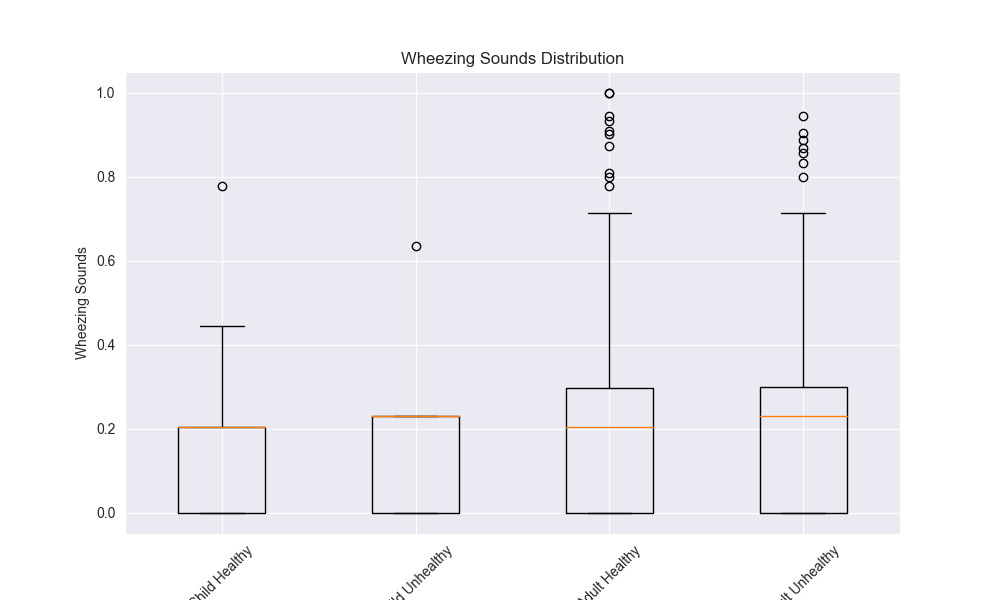
\includegraphics[width=0.35\textwidth]{wheezing.jpg}}
    \caption{Distribution of Cracking and Wheezing Sounds}
    \label{fig:unhealhty-distro}
\end{figure}

% The dataset was divided into healthy and unhealthy populations. Given these conditions, we were able to find the Average Cracking and Wheezing sound. This helped us understand the difference in the percentage of cracking and wheezing sounds in healthy bodies and unhealthy bodies at different age groups.

% All further analysis of numerical data was on the distribution of diseases. It was more sensible to analyse these based on sex and age. \\

%-------------------------------------------------------------------------
\section{Methodology}
The dataset provided sets of information in two forms - numerical and audio. All relevant information can be captured with the audio data.
Various machine learning models were trained using the numerical data and audio data separately to classify patients into eight categories, including healthy and seven specific COPDs.

\subsection*{Models on Numerical Data}
The classification based on the numerical data features extracted from the dataset served as baselines. The correlations among the numerical features, shown in Figure \ref{fig:corr} were relatively low, giving hope for practical baselines.

\begin{figure}[htbp]
    \centerline{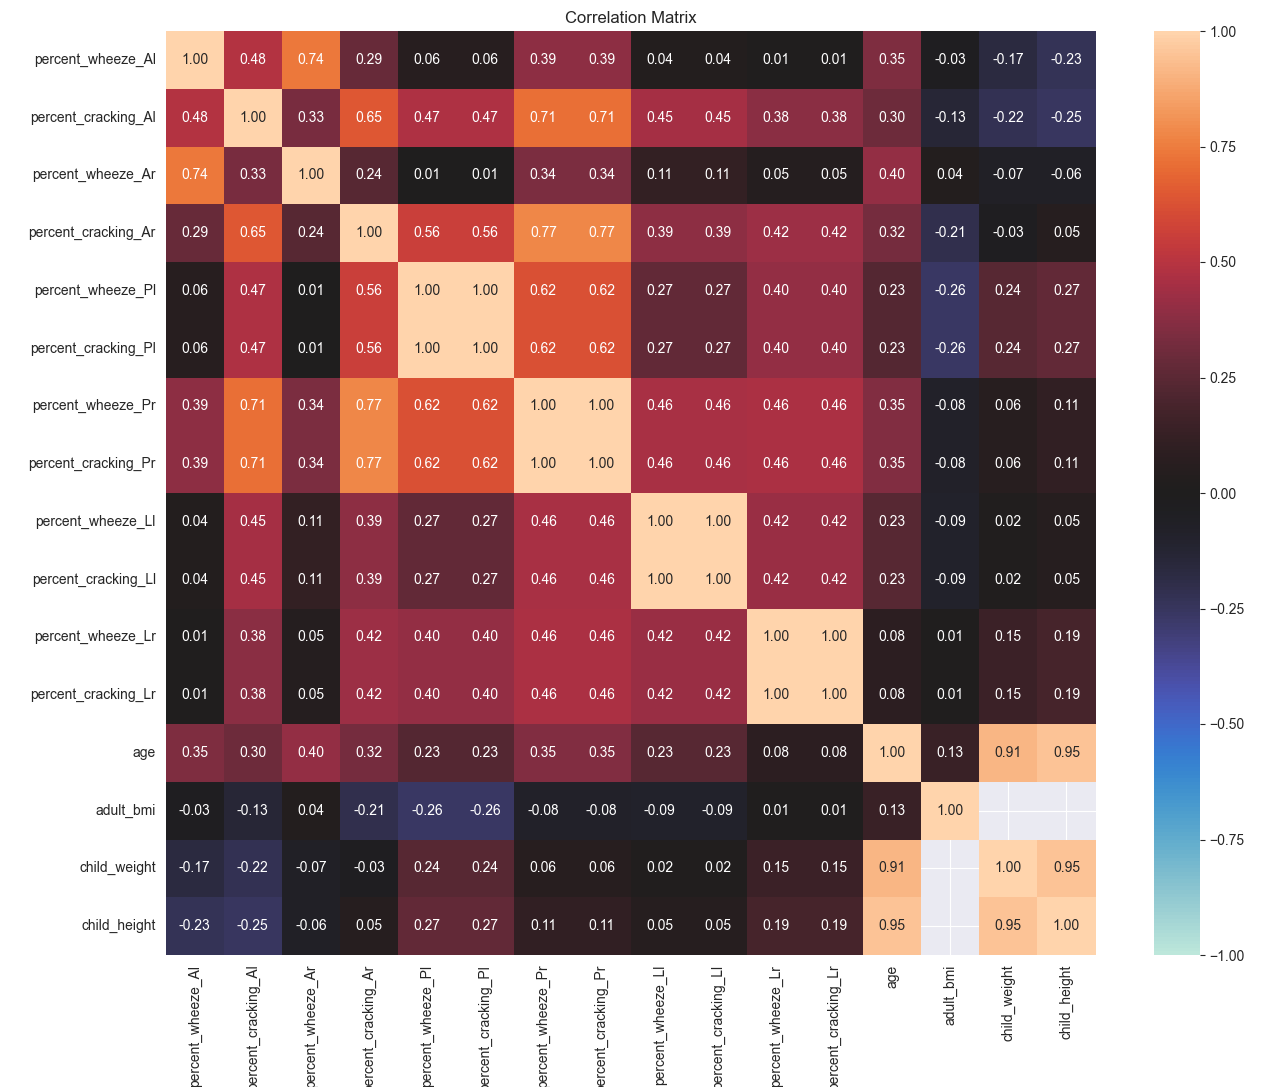
\includegraphics[width=0.5\textwidth]{corr.png}}
    \caption{Correlation Matrix for compressed numerical features}
    \label{fig:corr}
\end{figure}

Specifically, we showed that using only the numerical data, the Support Vector Machine model with Linear Kernel was above to achieve an overall accuracy of $\approx 0.8$ in the case of adults and children. Models trained on the numerical data enabled us to analyse the efficacy of using the presence of wheezing and crackling in a patient as markers of different COPDs. Since wheezing and crackling have been recorded as features in the given dataset, it is imperative to explore how 'difficult' it is to diagnose a person based on these features. Two distinct datasets were created for prediction: one for adults and another for children. This division was necessary because adult BMI data was unavailable for children, and conversely, child height and weight information was missing for adults. Consequently, separate classifiers were trained for each subset. Due to these variations in available features, creating a single model that could uniformly handle all data points wasn't feasible.
\\The accuracy for each model was validated using $k$-fold cross-validation with different values of $k$, including 3, 5, and 10. Even though we plan to analyse the models more intensely to find the scope for improvement, we believe that given a larger dataset, even such numerical features will produce a \textit{good enough} model. To verify the classifier's quality obtained, we also look at the models' precision, recall, and F1-score.

\subsection*{Models on Audio Data}
The audio pipeline contained the following steps:
\begin{enumerate}
    \item \textit{Preprocessing}:
    This included padding/truncating raw audio files to 20s of length.
    \item \textit{Augmentation}:
    To expand the audio dataset and make the models more robust to new data, augmentation was performed. This included:
    \begin{itemize}
        \item Random Noise: Addition of random noise to the audio files.
        \item Time Stretching: Stretching or compressing the audio files and padding them to 20s of length.
        \item Time Shifting: Moving the waveform in time, and wrapping it around the 20s window.
        \item Picth Shifting: Increasing/decreasing the pitch of the file.
    \end{itemize}
    The augmentation was performed randomly on all the files to create a new augmented dataset of size 920*5=4600 samples.
    \begin{figure}[htbp]
        \centerline{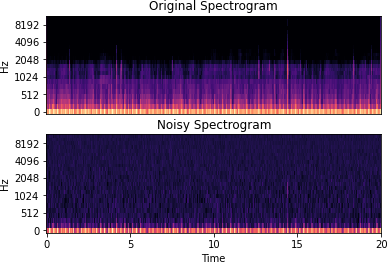
\includegraphics[width=0.35\textwidth]{Noisy.png}} \centerline{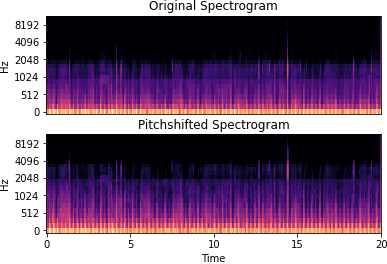
\includegraphics[width=0.35\textwidth]{Pitchshifted.png}} \centerline{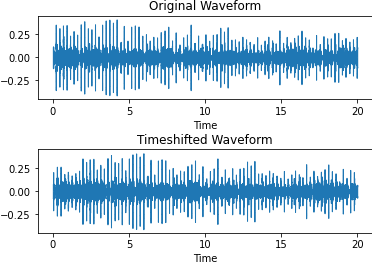
\includegraphics[width=0.35\textwidth]{timeshifted.png}} \centerline{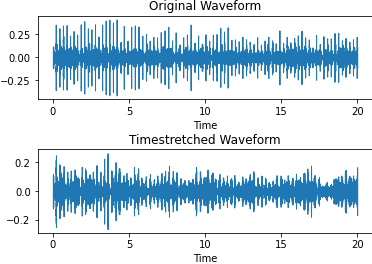
\includegraphics[width=0.35\textwidth]{Timestretched.png}}
        \caption{Augmented vs Original Audio for Patient 101}
        \label{fig:unhealhty}
    \end{figure}
    \item \textit{Feature Extraction}:
    This consisted of two steps:
    \begin{enumerate}
        \item Audio Feature Extraction: For extracting data from audio, the following were generated from each audio file:
        \begin{itemize}
            \item Mel Frequency Spectrogram
            \item MFCCs or Mel Frequency Cepstral Coefficients
            \item Chromagrams
            \item Chroma-Energy Normalised Statistics
        \end{itemize}
        These allowed us to represent the audio in a 2D numerical array, making them machine readable.
        \item Numerical Feature Extraction
        The audio features generated could be passed through a CNN to generate final set of numerical features by flattening its output, or simply flattened directly into a large-dimensional array.
    \end{enumerate}
    \item \textit{Classification}
    Classification was performed via the CNN by using the flattened features it output as inputs to an ANN. Meanwhile, the directly flattened features from the audio features were classified using the following models:
    \begin{itemize}
        \item SVM
        \item KNN
        \item Random Forest
        \item Logistic Regression
        \item Naive Bayes
    \end{itemize}
\end{enumerate}

\begin{figure}
    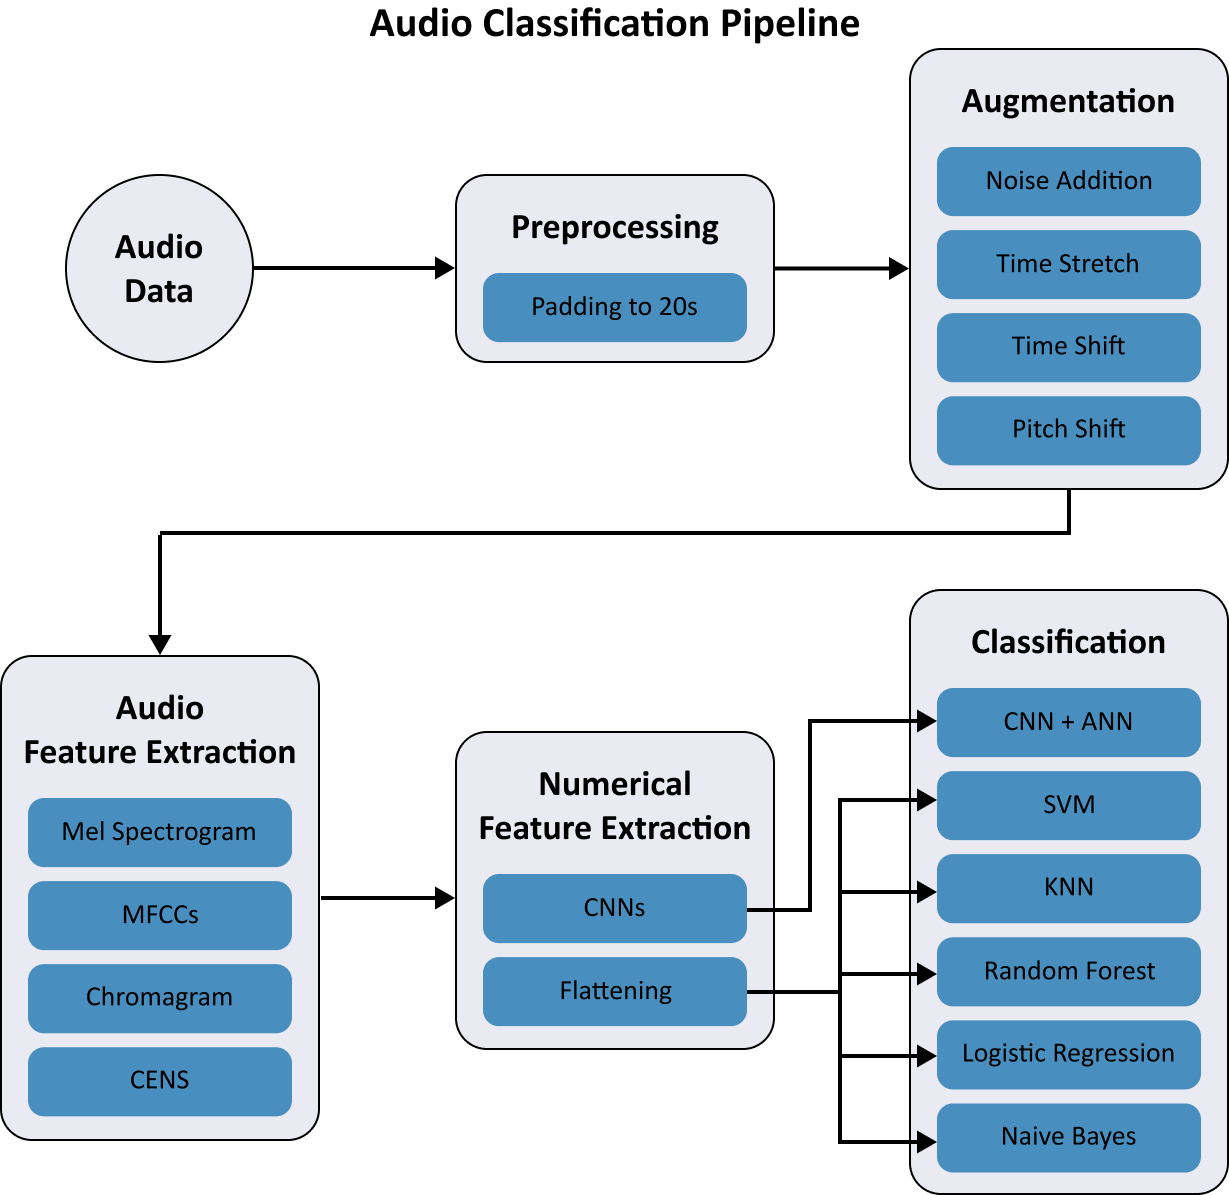
\includegraphics[scale=0.19]{Audio Pipeline.png}
    \caption{Pipeline used for developing classifiers using audio data}
    \label{fig:audio_pipeline}
\end{figure}

To train machine learning models to learn generalised patterns and classify the respiratory audio into one of eight categories, the first step required feature extraction from this audio. These features were extracted in the form of Mel Spectrograms, Mel-Frequency Cepstral Coefficients (MFCC) Spectrograms, Chromograms, and Chroma Energy Normalised Statistics (CENS), all of which condense the audio information into visual plots. These visual plots effectively converted the audio classification problem into an image classification problem for which we used multiple CNN-based models - one model for each type of image plot. The idea was to compare the discriminating power of these feature extraction methods and identify which method allowed the model to learn generalised patterns in the dataset most effectively.
\\All of these CNNs had a similar architecture - consisting sequentially of a convolution layer, a max-pooling layer, and another convolution layer, all three of which together perform the task of feature extraction from images followed by flattening the multi-dimensional representation matrix for each feature into a single vector. These layers were succeeded by three linear layers, which learn patterns from these flattened representations. Some parameters, such as the input and output sizes of the linear layers, were experimented with to cater to a specific type of feature set.
% Once we have the audio features given by Mel Spectrograms and CENS, which are essentially 2-dimensional arrays of values, we can use these as features and perform classification. Our literature review supports the claim to use CNNs for classification since the mapping from audios produces \textit{images}. However, on the run of training CNNs with the augmented data, it was seen that the CNN was too computationally expensive. Even with the features ready to feed into a CNN, we could not train a sufficient model on it due to resource constraints. Hence, we were forced to use the non-augmented dataset for the CNN.
% We use models trained on the non-augmented data for comparison since augmentation does not guarantee improvement. For the four instances of MFCC, Mel Spectrograms, Chromagrams, and CENS, we use a CNN architecture with a convolutional layer, max-pooling, and another convolutional layer. Finally, the architecture feeds the identified features into a fully connected network with hidden layers of sizes 256 and 64. Some parameters were fine-tuned to cater to a specific type of feature set.

A range of classifiers was tried for the problem on both the augmented and non-augmented flattened datasets, including SVMs, $k$-NN, and random forests.
% \begin{enumerate}
%     \item \textit{Gaussian Naive Bayes:}
%     Since the data distribution follows no pattern, statistical models like Naive Bayes are expected to fail. Moreover, our features are correlated - wheezing recorded from one position is not independent of the wheezing recorded in another position, violating the core assumption of Naive Bayes.
%     \item \textit{$k$-Nearest Neighbours:}
%     The $k$-NN model performs reasonably on the adult subset of the data; however, its performance is still poor on the children subset. This is likely due to the limited quantity of samples in the children's dataset, making it difficult for the model to learn enough discriminating features.
%     \item \textit{Decision Trees:}
%     The first D-Tree model was trained with Gini Impurity, with no particular pruning depth. This resulted in the model overfitting the data due to being \textit{too complex}. So, another tree was trained using Entropy with different pruning lengths for children and adults. This model performed well on the data.
%     \item \textit{Support Vector Machines:}
%     An SVM model trained with a linear kernel displayed the best performance of all models. SVMs are known to work well with smaller datasets. A decent performance also indicates that there exists a somewhat clear decision boundary in both subsets, which the SVM approximates as best as it can. These boundaries would hopefully be better with more data.
%     \item \textit{Logistic Regression:}
%     The simple logistic regression also works almost as well as the SVM model. Since the Linear SVM performed the best, we believe the data is linearly separable - hence, logistic regression performs decently well.
% \end{enumerate}

%-------------------------------------------------------------------------
\section{Results and Analysis}
\subsection*{Models on Numerical Data}
The lineup of models trained on numerical data included techniques from Gaussian Naive Bayes to Decision Trees and SVMs. A typical pattern is observed among all models - the prediction accuracy of children is generally lower than that of adults. This can be attributed to the fact that there are more adult training samples. Also, adults in the dataset have been classified into fewer classes (there are classes into which no adults have been classified). Similarly, fewer data points of children are classified into a larger number of classes - this is a consequence of having limited training data.

The performance of the models is tabulated in Table \ref{tab:performance}.

\begin{table}[htbp]
\resizebox{\linewidth}{!}{%
\centering
\begin{tabular}{c|llrlr}
\multirow{2}{*}{\textbf{S.No.}} & \multirow{2}{*}{\textbf{Model}} & \multicolumn{2}{c}{\textbf{Training Accuracy}} & \multicolumn{2}{c}{\textbf{Testing Accuracy}} \\
&                      & \textbf{Adult} & \textbf{Child} & \textbf{Adult} & \textbf{Child} \\ \hline
1 & \textit{Support Vector Machines}                  & \textbf{0.807}          & \textbf{0.55}           & \textbf{0.875}          & \textbf{0.6}            \\
2 & \textit{$k$-Nearest Neighbors}  & 0.836          & 0.403          & 0.75           & 0.4            \\
3 & \textit{Decision Trees}        & 0.752          & 0.4            & 0.625          & 0.6            \\
4 & \textit{Decision Trees}        & 0.721          & 0.649          & 0.75           & 0.6            \\
5 & \textit{(Gaussian) Naive Bayes} & 0.77           & 0.516          & 0.5            & 0.6            \\
6 & \textit{Logistic Regression}  & 0.838          & 0.514          & 0.875          & 0.6
\end{tabular}
}
\caption{Training and Testing Scores for Different Models}
\label{tab:performance}
\end{table}

The success of the logistic regression and SVM-based models can be used to infer the linear separability of the given data. This is further supported by the fact that the linear kernel function performed the best among the different kernel functions used for the SVM classifier. As previously stated, the SVM model with the linear kernel was the top performer. The slightly worse performance of logistic regression can be attributed to the increased robustness of SVMs to outliers.

% \begin{table}[htbp]
% \resizebox{\linewidth}{!}{%
% \centering
% \begin{tabular}{c|ll}
% \multirow{2}{*}{\textbf{S.No.}} & \multirow{2}{*}{\textbf{Model}} & \multirow{2}{*}{\textbf{Hyperparameters}} \\
%   &                      &                                                \\ \hline
% 1 & \textit{Support Vector Machines}                  & Linear Kernel                                  \\
% 2 & \textit{$k$-Nearest Neighbors}  & $k$ (Adults) = 10, $k$ (Children) = 5              \\
% 3 & \textit{Decision Trees}        & Gini Impurity, Max Depth = None                \\
% 4 & \textit{Decision Trees}        & Entropy, Max Depth = 10 (Adults), 5 (Children) \\
% 5 & \textit{(Gaussian) Naive Bayes} & Variable Smoothing: 1e-9                       \\
% 6 & \textit{Logistic Regression}  & Tolerance = 0.0001, Max Iterations = 5000
% \end{tabular}%
% }
% \caption{Hyperparameters used for the models in Table \ref{tab:performance}}
% \label{tab:hyperparams}
% \end{table}

% Our current challenge stems from limited data availability, preventing the training of an optimal model. However, we anticipate significant improvements when incorporating audio features into our classification process. Unlike binary numerical data, audio data offers richer information, potentially revealing various patterns beyond simple presence or absence. This expanded dataset allows our model to explore new patterns. The existing numerical model faces a time invariance issue due to the simplified representation of crackling and wheezing data. The audio-based model will overcome this limitation, offering a more comprehensive analysis without this constraint.
\subsection*{Models on Audio Data}
% With this, we intend to implement CNN-based models in the future to perform multi-class classification on Mel Spectrograms, MFCCs, and other features extracted from audio. We hope to overcome overfitting since we have a much larger audio data set. The literature study suggests that CNNs are a relatively common method of classification for audio data - a consequence of the layering of networks. Finally, a comprehensive model will be able to analyse both numerical and audio data to make its predictions.
As anticipated, extracting features directly from the respiratory audio and then performing multi-class classification on them yielded much better results than in the case of numerical data.

\begin{table}[htbp]
\resizebox{\linewidth}{!}{%
\centering
\begin{tabular}{c|lccc}
\multirow{2}{*}{\textbf{S.No.}} & \multirow{2}{*}{\textbf{Model}} & \multicolumn{3}{c}{\textbf{Accuracy}} \\
& & \textbf{Training} & \textbf{Validation} & \textbf{Testing} \\ \hline
1 & \textit{CNN on Spectrograms} & \textbf{0.874} & 0.815 & 0.815 \\
2 & \textit{CNN on MFCC} & 0.855 & \textbf{0.902} & \textbf{0.880} \\
3 & \textit{CNN on Chromagram} & 0.865 & 0.848 & 0.848 \\
4 & \textit{CNN on CENS} & 0.870 & 0.826 & 0.837 \\
\end{tabular}
}
\caption{Scores for different CNN Models}
\label{tab:performance-2}
\end{table}

The results for all CNN models have been tabulated in Table \ref{tab:performance-2} and visualized in Figure \ref{fig:cnn_accuracies}.

\begin{figure}[htbp]
\centering
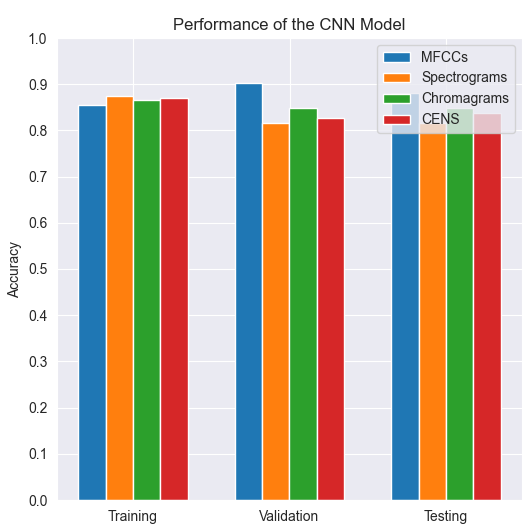
\includegraphics[scale=0.4]{cnn_accuracies.png} \\
\caption{Scores for different CNN Models}
\label{fig:cnn_accuracies}
\end{figure}

Models were created for the augmented audio datasets as well. However, the high computational requirements for training these models combined with our lack of resources to meet them, we were unable to actually train these models and evaluate the difference in performance brought on by augmenting the original dataset. It is important to note that according to our literature review, we anticipate an increase in performance due to augmentation.

The performance of other models trained on both augmented and non-augmented data can be seen in Figure \ref{fig:non-aug} and \ref{fig:aug}.
On a closer look, it is clear that the Support Vector Machine models trained using linear kernels outperform all others for most audio features.
\begin{figure}
    \centering
    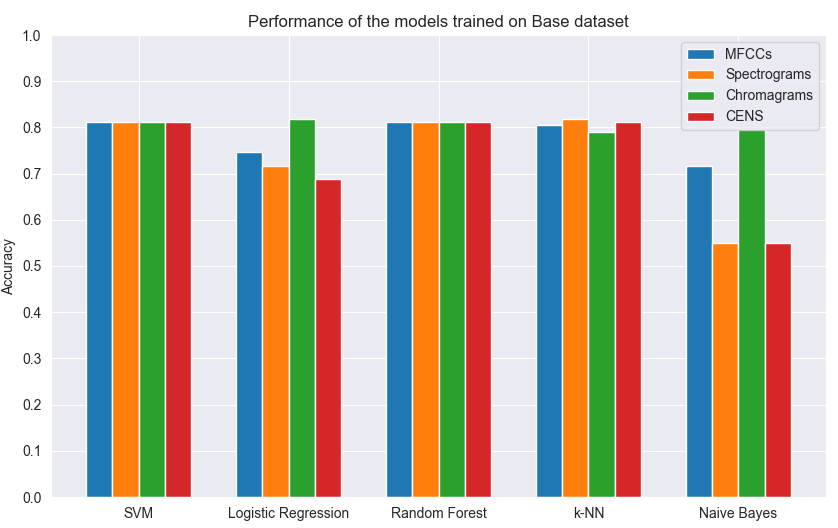
\includegraphics[scale=0.3]{non-aug_accuracies.png}
    \caption{Scores for models trained on non-augmented data}
    \label{fig:non-aug}
\end{figure}
\begin{figure}
    \centering
    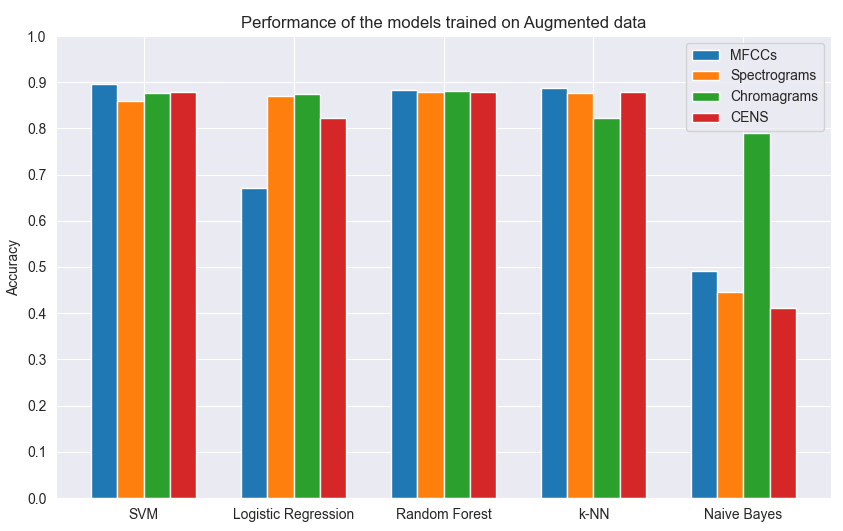
\includegraphics[scale=0.3]{aug_accuracies.png}
    \caption{Scores for models trained on augmented data}
    \label{fig:aug}
\end{figure}

%-------------------------------------------------------------------------
\section{Conclusion}

As per the proposal, we have created a model achieving an accuracy of 89.67\%, matching and, in fact, exceeding the accuracy of the most experienced medical professionals.

According to the analysis of machine learning techniques, This score was achieved by the SVM model trained on the augmented dataset with the MFCC-generated features.
Hence, we have improved upon our SVM-benchmark model which achieved a base score of around 0.8, trained on the numerical data. The spectrograms also show a contrast between healthy and unhealthy patients. So, we hope to make the classification more robust. The MFCCs consistently generated the best predictive features for classifiers.

Ultimately, we hope the model will enable more effective treatment and improve patient outcomes, using only basic numerical and audio data.

{\small
\bibliographystyle{ieee_fullname}
\bibliography{egbib}
}

\end{document}
